\documentclass[UTF8, 12pt]{ctexart}
\usepackage{color}
% 颜色
\definecolor{orange}{RGB}{255,127,0} 
\usepackage{amssymb}
% 因为所以
\usepackage{amsmath}
% 数学公式
\setcounter{tocdepth}{5}
\setcounter{secnumdepth}{5}
% 设置五级目录
\usepackage{geometry}
\geometry{papersize={21cm,29.7cm}}
\geometry{left=3.18cm,right=3.18cm,top=2.54cm,bottom=2.54cm}
% 设置页边距
\usepackage{indentfirst}
\setlength{\parindent}{2.45em}
% 设置首行缩进
\usepackage{setspace}
\renewcommand{\baselinestretch}{1.5}
% 设置行距
\usepackage{tikz}
% 绘图
\usepackage{xcolor}
% 为了实现不同的颜色
\usepackage{array}
% 设置表格行距
\usepackage{pifont}
% 圆圈序号
\author{Didnelpsun}
\title{考研数学准备}
\date{}
\begin{document}
\renewcommand
\arraystretch{1.5}
% 表格高1.5倍
\maketitle
\pagestyle{empty}
\thispagestyle{empty}
\tableofcontents
\thispagestyle{empty}
\newpage
\pagestyle{plain}
\setcounter{page}{1}
\section{函数的图像}
\subsection{直角坐标系图像}
\subsubsection{常见图像}
\paragraph{基本初等函数与初等函数} \leavevmode \bigskip

基本初等函数包括:常数函数、幂函数、指数函数、对数函数、三角函数、反三角函数。

\subparagraph{常数函数} \leavevmode \bigskip

$y=A$,A为常数,图像平行于x轴:

\begin{tikzpicture}[domain=-1:5]
    \draw[-latex](-1,0) -- (5,0) node[below]{$x$};
    \draw[-latex](0,-0.5) -- (0, 1.5) node[above]{$y$};
    \draw[black, thick](-1,1) -- (5,1) node[right]{$y=A$};
    \filldraw[black] (0,0) node[below]{$O$};
    \filldraw[black] (0,1) circle (2pt) node at(0.75,0.5){$(0,A)$};
\end{tikzpicture}

\subparagraph{幂函数} \leavevmode \bigskip

$y=x^{\mu}$,$\mu$为实数,当$x>0$,$y=x^{\mu}$都有定义:

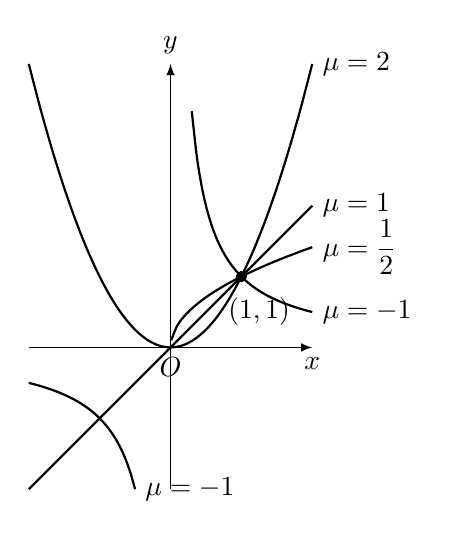
\begin{tikzpicture}[scale=0.9]
    \draw[-latex](-2,0) -- (2,0) node[below]{$x$};
    \draw[-latex](0,-2) -- (0,4) node[above]{$y$};
    \draw[black, thick, smooth, domain=0.3:2] plot (\x,1/\x) node[right]{$\mu =-1$};
    \draw[black, thick, smooth, domain=-2:-0.5] plot (\x,1/\x) node[right]{$\mu =-1$};
    \draw[black, thick, smooth, domain=0.01:2] plot (\x, {sqrt(\x)}) node[right]{$\mu =\dfrac{1}{2}$};
    \draw[black, thick, smooth, domain=-2:2] plot (\x,\x) node[right]{$\mu =1$};
    \draw[black, thick, smooth, domain=-2:2] plot (\x, {\x*\x}) node[right]{$\mu =2$};
    \filldraw[black] (0,0) node[below]{$O$};
    \filldraw[black] (1,1) circle (2pt) node at(1.25,0.5){$(1,1)$};
\end{tikzpicture}

所以对于幂函数,可以根据不同幂下相同单调性来研究最值:

\begin{enumerate}
    \item $\sqrt{u},\sqrt[3]{u}$可以使用$u$来研究。
    \item $\vert u\vert$可以使用$u^2$来研究。
    \item $\dfrac{1}{u},u>0$可以使用$u$来研究,但是最值相反。
    \item $u_1u_2...u_n$可以使用$\sum_{i=1}^{n}\ln u_i$来研究。
\end{enumerate}

\subparagraph{指数函数} \leavevmode \bigskip

$y=a^x(a>0,a\neq 1)$:

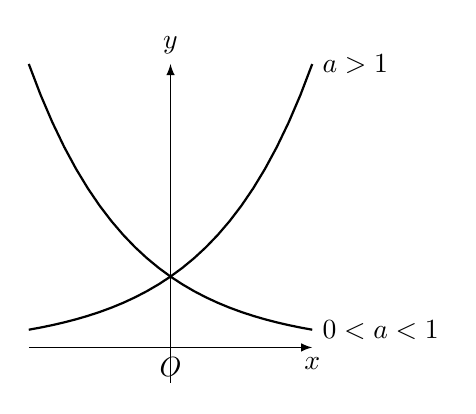
\begin{tikzpicture}[scale=0.9]
    \draw[-latex](-2,0) -- (2,0) node[below]{$x$};
    \draw[-latex](0,-0.5) -- (0,4) node[above]{$y$};
    \draw[black, thick, domain=-2:2] plot (\x,{pow(1/2,\x)}) node[right]{$0<a<1$};
    \draw[black, thick, domain=-2:2] plot (\x,{pow(2,\x)}) node[right]{$a>1$};
    \filldraw[black] (0,0) node[below]{$O$};
\end{tikzpicture}

指数函数具有如下性质:

\begin{enumerate}
    \item 特殊函数值:$a^0=1$。
    \item 定义域:$(-\infty, +\infty)$,值域:$(0,+\infty)$。
    \item 单调性:$a>1$,$y=a^x$单调增,$0<a<1$,$y=a^x$单调减。
    \item 常用指数函数:$y=e^x$。
    \item 极限:$\lim_{x\to -\infty}e^x=0$,$\lim_{x\to +\infty}e^x=+\infty$。
\end{enumerate}

\subparagraph{对数函数} \leavevmode \bigskip

$y=log_ax(a>0,a\neq 1)$为$y=a^x$的反函数:

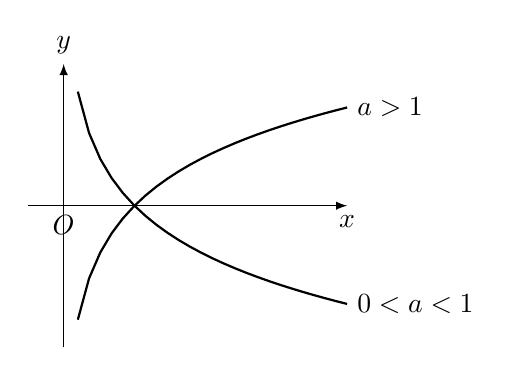
\begin{tikzpicture}[scale=0.9]
    \draw[-latex](-0.5,0) -- (4,0) node[below]{$x$};
    \draw[-latex](0,-2) -- (0,2) node[above]{$y$};
    \draw[black, thick, domain=0.2:4] plot (\x,{ln(1/\x)}) node[right]{$0<a<1$};
    \draw[black, thick, domain=0.2:4] plot (\x,{ln(\x)}) node[right]{$a>1$};
    \filldraw[black] (0,0) node[below]{$O$};
\end{tikzpicture}

对数函数具有如下性质:

\begin{enumerate}
    \item 特殊函数值:$\log_a1=0$,$log_aa=1,\ln 1=0,\ln e=1$。
    \item 定义域:$(0, +\infty)$,值域:$(-\infty,+\infty)$。
    \item 单调性:$a>1$,$y=\log_ax$单调增,$0<a<1$,$y=\log_ax$单调减。
    \item 常用对数函数:$y=\ln x$,$e=2.71828...$。
    \item 极限:$\lim_{x\to 0^+}\log_a x=-\infty$,$\lim_{x\to +\infty}\log_ax=+\infty$。
    \item 常用公式:$x=e^{\ln x}$,$u^v=e^{\ln u^v}=e^{v\ln u}(x>0,u>0)$
\end{enumerate}

\subparagraph{三角函数} \leavevmode \bigskip

正弦函数:

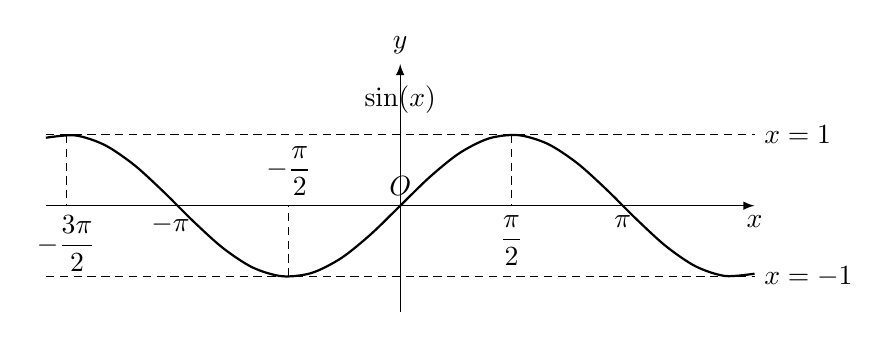
\begin{tikzpicture}[scale=0.9]
    \draw[-latex](-5,0) -- (5,0) node[below]{$x$};
    \draw[-latex](0,-1.5) -- (0,2) node[above]{$y$};
    \draw[black, thick, smooth, domain=-5:5] plot (\x,{sin(\x r)}) node at (0,1.5){$\sin(x)$};
    \draw[black, densely dashed](-5,1) -- (5,1) node[right]{$x=1$};
    \draw[black, densely dashed](-5,-1) -- (5,-1) node[right]{$x=-1$};
    \draw[black, densely dashed](-pi/2*3,1) -- (-pi/2*3,0) node[below]{$-\dfrac{3\pi}{2}$};
    \draw[black, densely dashed](-pi/2,-1) -- (-pi/2,0) node[above]{$-\dfrac{\pi}{2}$};
    \draw[black, densely dashed](pi/2,1) -- (pi/2,0) node[below]{$\dfrac{\pi}{2}$};
    \draw[black](0,0) -- (0,0) node[above]{$O$};
    \filldraw[black] (-pi-0.1,0) node[below]{$-\pi$};
    \filldraw[black] (pi,0) node[below]{$\pi$};
\end{tikzpicture}

余弦函数:

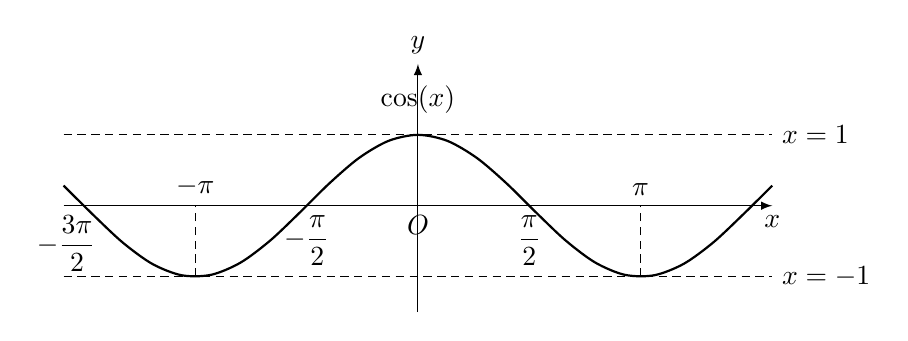
\begin{tikzpicture}[scale=0.9]
    \draw[-latex](-5,0) -- (5,0) node[below]{$x$};
    \draw[-latex](0,-1.5) -- (0,2) node[above]{$y$};
    \draw[black, thick, smooth, domain=-5:5] plot (\x,{cos(\x r)}) node at (0,1.5){$\cos(x)$};
    \draw[black, densely dashed](-5,1) -- (5,1) node[right]{$x=1$};
    \draw[black, densely dashed](-5,-1) -- (5,-1) node[right]{$x=-1$};
    \draw[black, densely dashed](-pi,-1) -- (-pi,0) node[above]{$-\pi$};
    \draw[black, densely dashed](pi,-1) -- (pi,0) node[above]{$\pi$};
    \filldraw[black] (0,0) node[below]{$O$};
    \filldraw[black] (-pi/2*3-0.25,0) node[below]{$-\dfrac{3\pi}{2}$};
    \filldraw[black] (-pi/2,0) node[below]{$-\dfrac{\pi}{2}$};
    \filldraw[black] (pi/2,0) node[below]{$\dfrac{\pi}{2}$};
\end{tikzpicture}

弦函数有如下特征:

\begin{enumerate}
    \item 特殊函数值:$\sin 0=0$,$\sin\dfrac{\pi}{6}=\dfrac{1}{2}$,$\sin\dfrac{\pi}{4}=\dfrac{\sqrt{2}}{2}$,$\sin\dfrac{\pi}{3}=\dfrac{\sqrt{3}}{2}$,$\sin\dfrac{\pi}{2}=1$,$\sin\pi=0$,$\sin\dfrac{3\pi}{2}=-1$,$\sin 2\pi=0$,$\cos 0=1$,$\cos\dfrac{\pi}{6}=\dfrac{\sqrt{3}}{2}$,$\cos\dfrac{\pi}{4}=\dfrac{\sqrt{2}}{2}$,$\cos\dfrac{\pi}{3}=\dfrac{1}{2}$,$\cos\dfrac{\pi}{2}=0$,$\cos\pi=-1$,$\cos\dfrac{3\pi}{2}=0$,$\cos 2\pi=1$。
    \item 定义域:$(-\infty, +\infty)$,值域:$[-1,+1]$。
    \item 奇偶性:$y=\sin x$为奇函数,$y=\cos x$为偶函数。
    \item 周期性:最小正周期为$2\pi$。
    \item 有界性:$\vert\sin x\vert\leqslant 1$,$\vert\cos x\vert\leqslant 1$。
\end{enumerate}

正切函数:

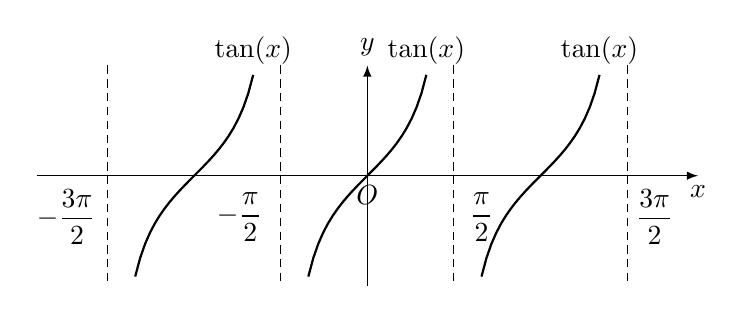
\begin{tikzpicture}[scale=0.7]
    \draw[-latex](-6,0) -- (6,0) node[below]{$x$};
    \draw[-latex](0,-2) -- (0,2) node[above]{$y$};
    \draw[black, thick, domain=-pi/2+0.5:pi/2-0.5] plot (\x,{tan(\x r)}) node[above]{$\tan(x)$};
    \draw[black, densely dashed](pi/2,2) -- (pi/2,-2);
    \draw[black, densely dashed](-pi/2,2) -- (-pi/2,-2);
    \draw[black, thick, domain=-pi/2*3+0.5:-pi/2-0.5] plot (\x,{tan(\x r)}) node[above]{$\tan(x)$};
    \draw[black, densely dashed](pi/2*3,2) -- (pi/2*3,-2);
    \draw[black, thick, domain=pi/2+0.5:pi/2*3-0.5] plot (\x,{tan(\x r)}) node[above]{$\tan(x)$};
    \draw[black, densely dashed](-pi/2*3,2) -- (-pi/2*3,-2);
    \filldraw[black] (0,0) node[below]{$O$};
    \filldraw[black] (pi/2+0.5,-0.75) node{$\dfrac{\pi}{2}$};
    \filldraw[black] (-pi/2-0.75,-0.75) node{$-\dfrac{\pi}{2}$};
    \filldraw[black] (pi/2*3+0.5,-0.75) node{$\dfrac{3\pi}{2}$};
    \filldraw[black] (-pi/2*3-0.75,-0.75) node{$-\dfrac{3\pi}{2}$};
\end{tikzpicture}

余切函数:

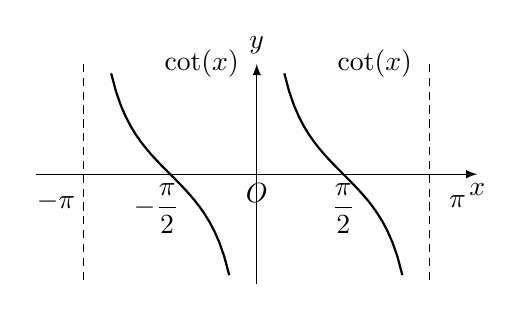
\begin{tikzpicture}[scale=0.7]
    \draw[-latex](-4,0) -- (4,0) node[below]{$x$};
    \draw[-latex](0,-2) -- (0,2) node[above]{$y$};
    \draw[black, thick, domain=0.5:pi-0.5] plot (\x,{cot(\x r)}) node at(pi-1,2){$\cot(x)$};
    \draw[black, densely dashed](pi,2) -- (pi,-2);
    \draw[black, thick, domain=-0.5:-pi+0.5] plot (\x,{cot(\x r)}) node at(-1,2){$\cot(x)$};
    \draw[black, densely dashed](-pi,2) -- (-pi,-2);
    \filldraw[black] (0,0) node[below]{$O$};
    \filldraw[black] (pi/2,0) node[below]{$\dfrac{\pi}{2}$};
    \filldraw[black] (pi+0.5,-0.5) node{$\pi$};
    \filldraw[black] (-pi/2-0.25,0) node[below]{$-\dfrac{\pi}{2}$};
    \filldraw[black] (-pi-0.5,-0.5) node{$-\pi$};
\end{tikzpicture}

切函数有如下特征:

\begin{enumerate}
    \item 特殊函数值:$\tan 0=0$,$\tan\frac{\pi}{6}=\frac{\sqrt{3}}{3}$,$\tan\frac{\pi}{4}=1$,$\tan\frac{\pi}{3}=\sqrt{3}$,$\lim_{x\to\frac{\pi}{2}}\tan x=\infty$,$\tan\pi=0$,$\lim_{x\to\frac{3\pi}{2}}\tan x=\infty$,$\tan 2\pi=0$,$\lim_{x\to 0}\cot x=\infty$,$\cot\dfrac{\pi}{6}=\sqrt{3}$,$\cot\dfrac{\pi}{4}=1$,$\cot\dfrac{\pi}{3}=\dfrac{\sqrt{3}}{3}$,$\cot\dfrac{\pi}{2}=0$,$\lim_{x\to\pi}\cot x=\infty$,$\cot\dfrac{3\pi}{2}=0$,$\lim_{x\to 2\pi}\cot x=\infty$。
    \item 定义域:$\tan x:x\neq k\pi+\dfrac{\pi}{2}(k\in Z)$,$\cot x:x\neq k\pi(k\in Z)$,值域:$(-\infty,+\infty)$。
    \item 奇偶性:定义域内均为奇函数。
    \item 周期性:最小正周期为$\pi$。
\end{enumerate}

$$
    \sec x=\dfrac{1}{\cos x},\csc x=\dfrac{1}{\sin x}
$$

正割函数:

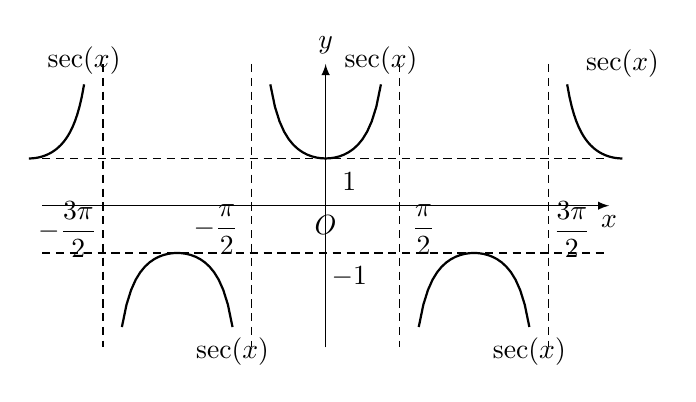
\begin{tikzpicture}[scale=0.6]
    \draw[-latex](-6,0) -- (6,0) node[below]{$x$};
    \draw[-latex](0,-3) -- (0,3) node[above]{$y$};
    \draw[black, thick, domain=-pi/2+0.4:pi/2-0.4] plot (\x,{sec(\x r)}) node[above]{$\sec(x)$};
    \draw[black, thick, domain=-pi/2*3+0.4:-pi/2-0.4] plot (\x,{sec(\x r)}) node[below]{$\sec(x)$};
    \draw[black, thick, domain=pi/2+0.4:pi/2*3-0.4] plot (\x,{sec(\x r)}) node[below]{$\sec(x)$};
    \draw[black, thick, domain=-pi*2:-pi/2*3-0.4] plot (\x,{sec(\x r)}) node[above]{$\sec(x)$};
    \draw[black, thick, domain=pi/2*3+0.4:pi*2] plot (\x,{sec(\x r)}) node at (pi*2,3){$\sec(x)$};
    \draw[black, densely dashed](-6,1) -- (6,1);
    \draw[black, densely dashed](-6,-1) -- (6,-1);
    \draw[black, densely dashed](-pi/2*3,3) -- (-pi/2*3,-3);
    \draw[black, densely dashed](-pi/2,3) -- (-pi/2,-3);
    \draw[black, densely dashed](pi/2,3) -- (pi/2,-3);
    \draw[black, densely dashed](pi/2*3,3) -- (pi/2*3,-3);
    \filldraw[black] (0,0) node[below]{$O$};
    \filldraw[black] (0.5,0.5) node{$1$};
    \filldraw[black] (0.5,-1.5) node{$-1$};
    \filldraw[black] (-pi/2*3-0.75,-0.5) node{$-\dfrac{3\pi}{2}$};
    \filldraw[black] (-pi/2-0.75,-0.5) node{$-\dfrac{\pi}{2}$};
    \filldraw[black] (pi/2+0.5,-0.5) node{$\dfrac{\pi}{2}$};
    \filldraw[black] (pi/2*3+0.5,-0.5) node{$\dfrac{3\pi}{2}$};
\end{tikzpicture}

余割函数:

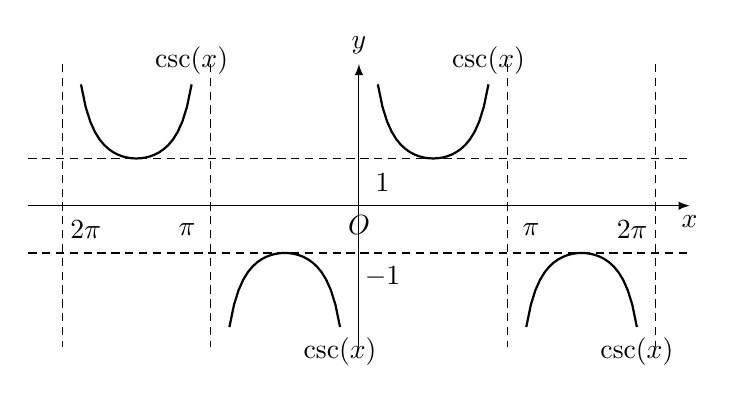
\begin{tikzpicture}[scale=0.6]
    \draw[-latex](-7,0) -- (7,0) node[below]{$x$};
    \draw[-latex](0,-3) -- (0,3) node[above]{$y$};
    \draw[black, thick, domain=0.4:pi-0.4] plot (\x,{1/sin(\x r)}) node[above]{$\csc(x)$};
    \draw[black, thick, domain=pi+0.4:pi*2-0.4] plot (\x,{1/sin(\x r)}) node[below]{$\csc(x)$};
    \draw[black, thick, domain=-pi+0.4:-0.4] plot (\x,{1/sin(\x r)}) node[below]{$\csc(x)$};
    \draw[black, thick, domain=-pi*2+0.4:-pi-0.4] plot (\x,{1/sin(\x r)}) node[above]{$\csc(x)$};
    \draw[black, densely dashed](-7,1) -- (7,1);
    \draw[black, densely dashed](-7,-1) -- (7,-1);
    \draw[black, densely dashed](-pi,3) -- (-pi,-3);
    \draw[black, densely dashed](-pi*2,3) -- (-pi*2,-3);
    \draw[black, densely dashed](pi,3) -- (pi,-3);
    \draw[black, densely dashed](pi*2,3) -- (pi*2,-3);
    \filldraw[black] (0,0) node[below]{$O$};
    \filldraw[black] (0.5,0.5) node{$1$};
    \filldraw[black] (0.5,-1.5) node{$-1$};
    \filldraw[black] (-pi-0.5,-0.5) node{$\pi$};
    \filldraw[black] (-pi*2+0.5,-0.5) node{$2\pi$};
    \filldraw[black] (pi+0.5,-0.5) node{$\pi$};
    \filldraw[black] (pi*2-0.5,-0.5) node{$2\pi$};
\end{tikzpicture}

割函数有如下特征:

\begin{enumerate}
    \item 定义域:$\sec x:x\neq k\pi+\dfrac{\pi}{2}(k\in Z)$,$\csc x:x\neq k\pi(k\in Z)$,值域:$(-\infty,-1]\cup [1,+\infty)$。
    \item 奇偶性:$y=\sec x$为偶函数,$y=\csc x$为奇函数。
    \item 周期性:最小正周期为$2\pi$。
\end{enumerate}

\subparagraph{反三角函数} \leavevmode \bigskip

反正弦函数:

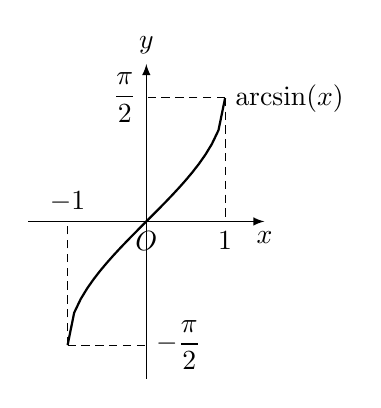
\begin{tikzpicture}
    \draw[-latex](-1.5,0) -- (1.5,0) node[below]{$x$};
    \draw[-latex](0,-2) -- (0,2) node[above]{$y$};
    \draw[black, thick, domain=-1:1] plot (\x,{rad(asin(\x))}) node[right]{$\arcsin(x)$};
    \draw[black, densely dashed](1,pi/2) -- (0,pi/2) node[left]{$\dfrac{\pi}{2}$};
    \filldraw[black] (0,0) node[below]{$O$};
    \draw[black, densely dashed](1,pi/2) -- (1,0) node[below]{$1$};
    \draw[black, densely dashed](-1,-pi/2) -- (0,-pi/2) node[right]{$-\dfrac{\pi}{2}$};
    \draw[black, densely dashed](-1,-pi/2) -- (-1,0) node[above]{$-1$};
\end{tikzpicture}

反余弦函数:

\begin{tikzpicture}
    \draw[-latex](-1.5,0) -- (1.5,0) node[below]{$x$};
    \draw[-latex](0,-0.5) -- (0,4) node[above]{$y$};
    \draw[black, thick, domain=-1:1] plot (\x,{rad(acos(\x)}) node at (-2, pi){$\arccos(x)$};
    \filldraw[black] (0,pi/2+0.5) node[right]{$\dfrac{\pi}{2}$};
    \draw[black](1,0) -- (1,0) node[below]{$1$};
    \filldraw[black] (0,0) node[below]{$O$};
    \draw[black, densely dashed](-1,pi) -- (0,pi) node[right]{$\pi$};
    \draw[black, densely dashed](-1,pi) -- (-1,0) node[below]{$-1$};
\end{tikzpicture}

反弦函数有如下特征:

\begin{enumerate}
    \item 特殊函数值:$\arcsin 0=0$,$\arcsin\dfrac{1}{2}=\dfrac{\pi}{6}$,$\arcsin\dfrac{\sqrt{2}}{2}=\dfrac{\pi}{4}$,$\arcsin\dfrac{\sqrt{3}}{2}=\dfrac{\pi}{3}$,$\arcsin 1=\dfrac{\pi}{2}$,$\arccos 1=0$,$\arccos\dfrac{\sqrt{3}}{2}=\dfrac{\pi}{6}$,$\arccos\dfrac{\sqrt{2}}{2}=\dfrac{\pi}{4}$,$\arccos\dfrac{1}{2}=\dfrac{\pi}{3}$,$\arccos 0=\dfrac{\pi}{2}$。
    \item 定义域:$(-1, +1)$,值域:$\arcsin x:[-\dfrac{\pi}{2},+\dfrac{\pi}{2}]$,$\arccos x:[0,\pi]$。
    \item 单调性:$y=\arcsin x$单调增,$y=\arccos x$单调减。
    \item 奇偶性:$y=\arcsin x$为奇函数。
    \item 有界性:$\vert\arcsin x\vert\leqslant\dfrac{\pi}{2}$,$0\leqslant\arccos x\leqslant\pi$。
    \item 性质:$\arcsin x+\arccos x=\dfrac{\pi}{2}(-1\leqslant x\leqslant 1)$
\end{enumerate}

对反弦函数性质进行证明:

令$f(x)=\arcsin x+\arccos x$,对其求导得:$f'(x)=\dfrac{1}{\sqrt{1-x^2}}-\dfrac{1}{1-x^2}=0$,所以$f(x)$是个常数函数。

又$f(0)=\dfrac{\pi}{2}$,所以该函数等于$\dfrac{\pi}{2}$。

反正切函数:

\begin{tikzpicture}[scale=0.9]
    \draw[-latex](-3,0) -- (3,0) node[below]{$x$};
    \draw[-latex](0,-2) -- (0,2) node[above]{$y$};
    \draw[black, thick, domain=-3:3] plot (\x,{rad(atan(\x))}) node[right]{$\arctan(x)$};
    \filldraw[black] (0,0) node[below]{$O$};
    \draw[black, densely dashed](-3,pi/2) -- (3,pi/2);
    \draw[black, densely dashed](-3,-pi/2) -- (3,-pi/2);
    \filldraw[black] (0.5,pi/2-0.5) node{$\dfrac{\pi}{2}$};
    \filldraw[black] (0.5,-pi/2-0.5) node{$-\dfrac{\pi}{2}$};
\end{tikzpicture}

反余切函数:

\begin{tikzpicture}[scale=0.9]
    \draw[-latex](-3,0) -- (3,0) node[below]{$x$};
    \draw[-latex](0,-0.5) -- (0,4) node[above]{$y$};
    \draw[black, thick, domain=-3:3] plot (\x,{pi/2-rad(atan(\x))}) node[right]{$\rm{arccot}(\textit{x})$};
    \filldraw[black] (0,0) node[below]{$O$};
    \draw[black, densely dashed](-3,pi) -- (3,pi);
    \filldraw[black] (-0.5,pi/2-0.5) node{$\dfrac{\pi}{2}$};
\end{tikzpicture}

反切函数有如下特征:

\begin{enumerate}
    \item 特殊函数值:$\arctan 0=0$,$\arctan\dfrac{\pi}{6}=\dfrac{\sqrt{3}}{3}=$,$\arctan 1=\dfrac{\pi}{4}$,$\arctan\sqrt{3}=\dfrac{\pi}{3}$,$\rm{arccot}0=\dfrac{\pi}{2}$,$\rm{arccot}\sqrt{3}=\dfrac{\pi}{6}$,$\rm{arccot}1=\dfrac{\pi}{4}$,$\rm{arccot}\dfrac{\sqrt{3}}{3}=\dfrac{\pi}{3}$。
    \item 定义域:$(-\infty, +\infty)$,值域:$\arctan x:[-\dfrac{\pi}{2},+\dfrac{\pi}{2}]$,$\rm{arccot}\,\textit{x}:[0,\pi]$。
    \item 单调性:$y=\arctan x$单调增,$y=\rm{arccot}x$单调减。
    \item 奇偶性:$y=\arctan x$为奇函数。
    \item 有界性:$\vert\arctan x\vert\leqslant\dfrac{\pi}{2}$,$0\leqslant\rm{arccot}\,\textit{x}\leqslant\pi$。
    \item 性质:$\arctan x+\rm{arccot}\,\textit{x}=\dfrac{\pi}{2}(-\infty<x<+\infty)$
\end{enumerate}

\subparagraph{初等函数} \leavevmode \bigskip

由基本初等函数经过有限次四则运算与符合步骤且可以被一个式子所表示。

幂指函数$u(x)^{v(x)}=e^{v(x)\ln u(x)}$也是初等函数。

\paragraph{分段函数} \leavevmode \bigskip

x的不同范围对应不同的法则,经典形式如下:

\begin{equation}\notag
    f(x)=\left\{ \begin{array}{lcl}
        \psi_1(x), &  & x>x_0 \\
        a,         &  & x=x_0 \\
        \psi_2(x), &  & x<x_0
    \end{array}
    \right.
    \text{或}f(x)=\left\{ \begin{array}{clc}
        \psi(x), &  & x\neq x_0 \\
        a,       &  & x=x_0
    \end{array}
    \right.
\end{equation}

\subparagraph{绝对值函数} \leavevmode \bigskip

$
    y=\vert x\vert=\left\{
    \begin{array}{lcl}
        x,  &  & x\geqslant 0 \\
        -x, &  & x<0
    \end{array}
    \right.
$

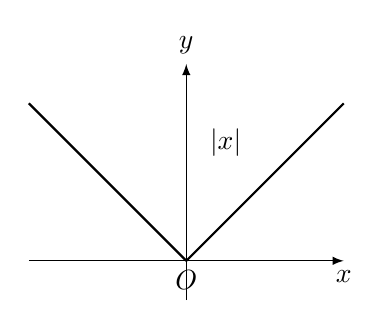
\begin{tikzpicture}
    \draw[-latex](-2,0) -- (2,0) node[below]{$x$};
    \draw[-latex](0,-0.5) -- (0,2.5) node[above]{$y$};
    \draw[black, thick, domain=0:2] plot (\x,\x);
    \draw[black, thick, domain=-2:0] plot (\x,-\x);
    \filldraw[black] (0.5,1.5) node{$\vert x\vert$};
    \filldraw[black] (0,0) node[below]{$O$};
\end{tikzpicture}

\subparagraph{符号函数} \leavevmode \bigskip

$
    y=\rm{sgn}x=\left\{
    \begin{array}{lcl}
        1,  &  & x>0 \\
        0,  &  & x=0 \\
        -1, &  & x<0
    \end{array}
    \right.
$

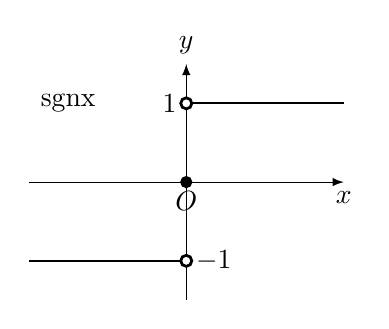
\begin{tikzpicture}
    \draw[-latex](-2,0) -- (2,0) node[below]{$x$};
    \draw[-latex](0,-1.5) -- (0,1.5) node[above]{$y$};
    \draw[black, thick, domain=0:2] plot (\x,1);
    \draw[black, thick, domain=-2:0] plot (\x,-1);
    \filldraw[black] (-1.5,1) node{$\rm{sgn}x$};
    \filldraw[black] circle (2pt) (0,0) node[below]{$O$};
    \filldraw[white, draw=black, line width=1pt] (0,1) circle (2pt);
    \filldraw[black] (0,1) node[left]{$1$};
    \filldraw[white, draw=black, line width=1pt] (0,-1) circle (2pt);
    \filldraw[black] (0,-1) node[right]{$-1$};
\end{tikzpicture}

\subparagraph{取整函数} \leavevmode \bigskip

$x$为实数,不超过$x$的最大整数称为其整数部分$[x]$,其定义域为$R$,值域为$Z$。

\begin{enumerate}
    \item $x-1<[x]\leqslant x$。
    \item $\lim_{x\to 0^+}[x]=0$。
    \item $\lim_{x\to 0^-}[x]=-1$。
\end{enumerate}

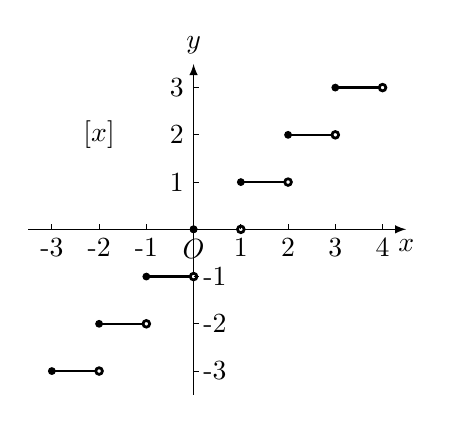
\begin{tikzpicture}[scale=0.6]
    \draw[-latex](-3.5,0) -- (4.5,0) node[below]{$x$};
    \draw[-latex](0,-3.5) -- (0,3.5) node[above]{$y$};
    \draw[black, thick, domain=1:2] plot (\x,1);
    \draw[black, thick, domain=2:3] plot (\x,2);
    \draw[black, thick, domain=3:4] plot (\x,3);
    \draw[black, thick, domain=-1:0] plot (\x,-1);
    \draw[black, thick, domain=-2:-1] plot (\x,-2);
    \draw[black, thick, domain=-3:-2] plot (\x,-3);
    \filldraw[black] (-2,2) node{$[x]$};
    \filldraw[black] circle (2pt) (0,0) node[below]{$O$};
    \foreach \x in {-2,...,4}
    \filldraw[white, draw=black, line width=1pt] (\x,\x-1) circle (2pt);
    \foreach \x in {3,...,-3}
    \filldraw[black] (\x,\x) circle (2pt);
    \foreach \x/\xtext in {-3,...,-1}
    \filldraw[black] (\x,0) node[below]{\xtext} -- ++(0, 3pt);
    \foreach \x/\xtext in {1,...,4}
    \filldraw[black] (\x,0) node[below]{\xtext} -- ++(0, 3pt);
    \foreach \x/\xtext in {1,...,3}
    \filldraw[black] (0,\x) node[left]{\xtext} -- +(3pt, 0);
    \foreach \x/\xtext in {-3,...,-1}
    \filldraw[black] (0,\x) node[right]{\xtext} -- +(3pt, 0);
\end{tikzpicture}

\subsubsection{图像变换}
\paragraph{平移变换}
\subparagraph{左右平移} \leavevmode \bigskip

$f(x)$沿$x$轴左移$x_0$个单位长度得到$f(x+x_0)$,向右移动$x_0$个单位则得到$f(x-x_0)$:

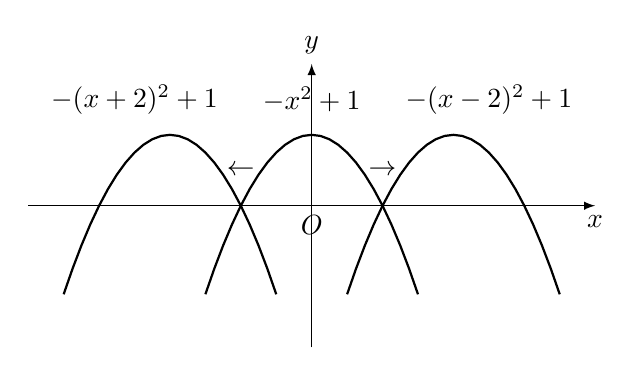
\begin{tikzpicture}[scale=0.9]
    \draw[-latex](-4,0) -- (4,0) node[below]{$x$};
    \draw[-latex](0,-2) -- (0,2) node[above]{$y$};
    \filldraw[black] (0,0) node[below]{$O$};
    \draw[black, thick, domain=-1.5:1.5] plot (\x,-\x*\x+1);
    \filldraw[black] (0,1.5) node{$-x^2+1$};
    \draw[black, thick, domain=0.5:3.5] plot (\x,{-pow((\x-2),2)+1});
    \filldraw[black] (2.5,1.5) node{$-(x-2)^2+1$};
    \draw[black, thick, domain=-3.5:-0.5] plot (\x,{-pow((\x+2),2)+1});
    \filldraw[black] (-2.5,1.5) node{$-(x+2)^2+1$};
    \filldraw[black] (1,0.5) node{$\rightarrow$};
    \filldraw[black] (-1,0.5) node{$\leftarrow$};
\end{tikzpicture}

\subparagraph{上下平移} \leavevmode \bigskip

$f(x)$沿$y$轴上移$y_0$个单位长度得到$f(x)+y_0$,向下移动$y_0$个单位则得到$f(x)-y_0$:

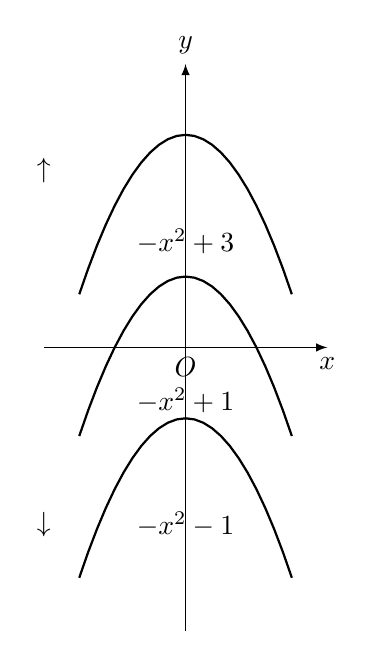
\begin{tikzpicture}[scale=0.9]
    \draw[-latex](-2,0) -- (2,0) node[below]{$x$};
    \draw[-latex](0,-4) -- (0,4) node[above]{$y$};
    \filldraw[black] (0,0) node[below]{$O$};
    \draw[black, thick, domain=-1.5:1.5] plot (\x,-\x*\x+1);
    \filldraw[black] (0,-0.75) node{$-x^2+1$};
    \draw[black, thick, domain=-1.5:1.5] plot (\x,{-\x*\x+3});
    \filldraw[black] (0,1.5) node{$-x^2+3$};
    \draw[black, thick, domain=-1.5:1.5] plot (\x,{-\x*\x+-1});
    \filldraw[black] (0,-2.5) node{$-x^2-1$};
    \filldraw[black] (-2,2.5) node{$\uparrow $};
    \filldraw[black] (-2,-2.5) node{$\downarrow $};
\end{tikzpicture}

\paragraph{对称变换}
\subparagraph{上下对称} \leavevmode \bigskip

将$f(x)$关于$x$轴对称得到$-f(x)$:

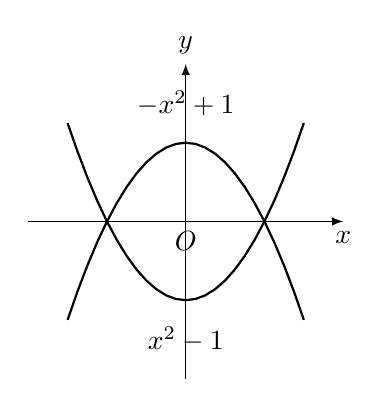
\begin{tikzpicture}
    \draw[-latex](-2,0) -- (2,0) node[below]{$x$};
    \draw[-latex](0,-2) -- (0,2) node[above]{$y$};
    \filldraw[black] (0,0) node[below]{$O$};
    \draw[black, thick, domain=-1.5:1.5] plot (\x,-\x*\x+1);
    \filldraw[black] (0,1.5) node{$-x^2+1$};
    \draw[black, thick, domain=-1.5:1.5] plot (\x,\x*\x-1);
    \filldraw[black] (0,-1.5) node{$x^2-1$};
\end{tikzpicture}

\subparagraph{左右对称} \leavevmode \bigskip

将$f(x)$关于$y$轴对称得到$f(-x)$:

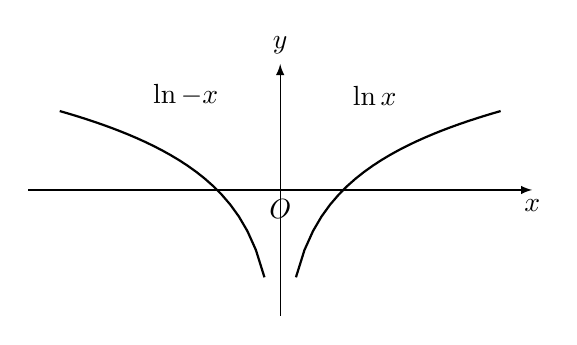
\begin{tikzpicture}[scale=0.8]
    \draw[-latex](-4,0) -- (4,0) node[below]{$x$};
    \draw[-latex](0,-2) -- (0,2) node[above]{$y$};
    \filldraw[black] (0,0) node[below]{$O$};
    \draw[black, thick, domain=0.25:3.5] plot (\x,{ln(\x)});
    \filldraw[black] (1.5,1.5) node{$\ln x$};
    \draw[black, thick, domain=-0.25:-3.5] plot (\x,{ln(-\x)});
    \filldraw[black] (-1.5,1.5) node{$\ln -x$};
\end{tikzpicture}

\subparagraph{原点对称} \leavevmode \bigskip

将$f(x)$关于$x$轴$y$轴即关于原点对称得到$-f(-x)$:

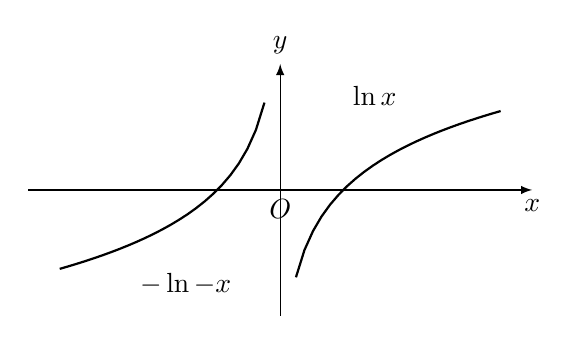
\begin{tikzpicture}[scale=0.8]
    \draw[-latex](-4,0) -- (4,0) node[below]{$x$};
    \draw[-latex](0,-2) -- (0,2) node[above]{$y$};
    \filldraw[black] (0,0) node[below]{$O$};
    \draw[black, thick, domain=0.25:3.5] plot (\x,{ln(\x)});
    \filldraw[black] (1.5,1.5) node{$\ln x$};
    \draw[black, thick, domain=-0.25:-3.5] plot (\x,{-ln(-\x)});
    \filldraw[black] (-1.5,-1.5) node{$-\ln -x$};
\end{tikzpicture}

\subparagraph{反函数对称} \leavevmode \bigskip

将$f(x)$关于$y=x$轴对称得到$f^{-1}(x)$:

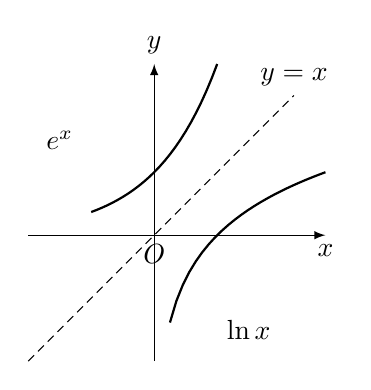
\begin{tikzpicture}[scale=0.8]
    \draw[-latex](-2,0) -- (e,0) node[below]{$x$};
    \draw[-latex](0,-2) -- (0,e) node[above]{$y$};
    \filldraw[black] (0,0) node[below]{$O$};
    \draw[black, thick, domain=0.25:e] plot (\x,{ln(\x)});
    \filldraw[black] (1.5,-1.5) node{$\ln x$};
    \draw[black, thick, domain=-1:1] plot (\x,{exp(\x)});
    \filldraw[black] (-1.5,1.5) node{$e^x$};
    \draw[black, densely dashed] (-2,-2) -- (e-0.5,e-0.5) node[above]{$y=x$};
\end{tikzpicture}

\subparagraph{函数绝对值} \leavevmode \bigskip

保留$f(x)$函数值在$[0,\infty]$的部分,并对$[-\infty,0]$部分进行上下对称:

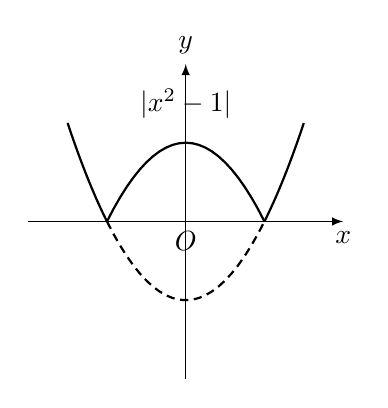
\begin{tikzpicture}
    \draw[-latex](-2,0) -- (2,0) node[below]{$x$};
    \draw[-latex](0,-2) -- (0,2) node[above]{$y$};
    \filldraw[black] (0,0) node[below]{$O$};
    \draw[black, thick, domain=1:1.5] plot (\x,\x*\x-1);
    \draw[black, thick, densely dashed, domain=-1:1] plot (\x,\x*\x-1);
    \draw[black, thick, domain=-1:1] plot (\x,-\x*\x+1);
    \draw[black, thick, domain=-1.5:-1] plot (\x,\x*\x-1);
    \filldraw[black] (0,1.5) node{$\vert x^2-1\vert$};
\end{tikzpicture}

\subparagraph{自变量绝对值} \leavevmode \bigskip

先只保留$f(x)$定义域在$[0,\infty]$的部分,然后在$[-\infty,0]$部分使用$[0,\infty]$的部分进行左右对称:

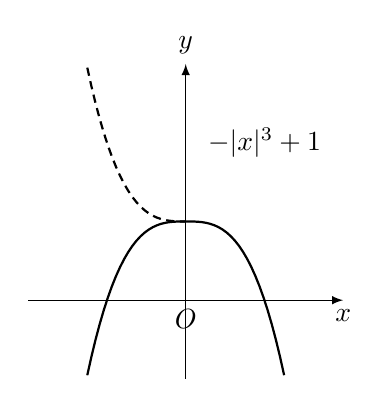
\begin{tikzpicture}
    \draw[-latex](-2,0) -- (2,0) node[below]{$x$};
    \draw[-latex](0,-1) -- (0,3) node[above]{$y$};
    \filldraw[black] (0,0) node[below]{$O$};
    \draw[black, thick, domain=0:1.25] plot (\x,{-pow(\x,3)+1});
    \draw[black, thick, densely dashed, domain=-1.25:0] plot (\x,{-pow(\x,3)+1});
    \draw[black, thick, domain=-1.25:0] plot (\x,{-pow(-\x,3)+1});
    \filldraw[black] (1,2) node{$-\vert x\vert^3+1$};
\end{tikzpicture}

\paragraph{伸缩变换}
\subparagraph{水平伸缩} \leavevmode \bigskip

纵坐标不变,当$k>1$时,$y=f(kx)$是$y=f(x)$缩短k倍得到,当$0<k<1$时,$y=f(kx)$是$y=f(x)$伸长k倍得到:

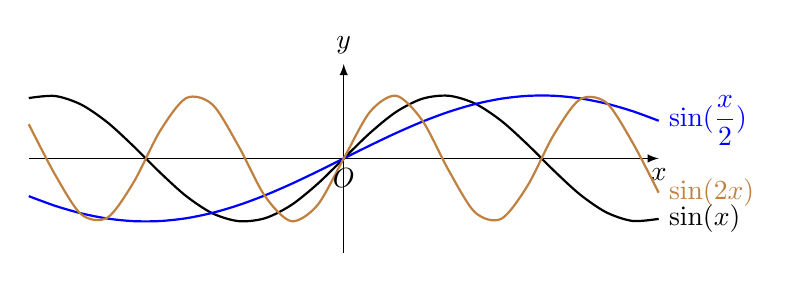
\begin{tikzpicture}[scale=0.8]
    \draw[-latex](-5,0) -- (5,0) node[below]{$x$};
    \draw[-latex](0,-1.5) -- (0,1.5) node[above]{$y$};
    \draw[black, thick, smooth, domain=-5:5] plot (\x,{sin(\x r)}) node[right]{$\sin(x)$};
    \draw[blue, thick, smooth, domain=-5:5] plot (\x,{sin(\x/2 r)}) node[right]{$\sin(\dfrac{x}{2})$};
    \draw[brown, thick, smooth, domain=-5:5] plot (\x,{sin(\x*2 r)}) node[right]{$\sin(2x)$};
    \filldraw[black] (0,0) node[below]{$O$};
\end{tikzpicture}


\subparagraph{垂直伸缩} \leavevmode \bigskip

横坐标不变,$y=kf(x)$的对应纵坐标为$y=f(x)$对应纵坐标的$k$倍。

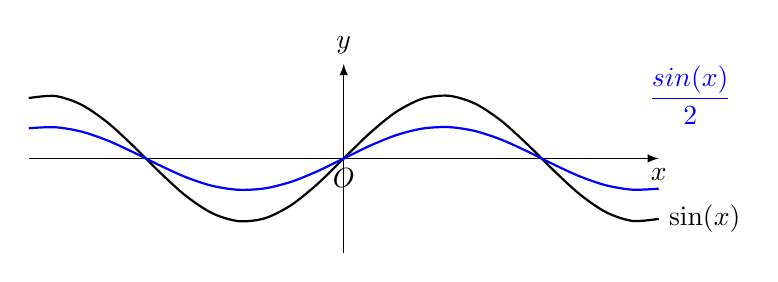
\begin{tikzpicture}[scale=0.8]
    \draw[-latex](-5,0) -- (5,0) node[below]{$x$};
    \draw[-latex](0,-1.5) -- (0,1.5) node[above]{$y$};
    \draw[black, thick, smooth, domain=-5:5] plot (\x,{sin(\x r)}) node[right]{$\sin(x)$};
    \draw[blue, thick, smooth, domain=-5:5] plot (\x,{sin(\x r)/2}) node at(5.5,1){$\dfrac{sin(x)}{2}$};
    \filldraw[black] (0,0) node[below]{$O$};
\end{tikzpicture}

\subsection{极坐标系图像}
\subsubsection{描点法}
\paragraph{心形线(外摆线)} \leavevmode \bigskip

心形线又称为心脏线,表示是一个圆上的固定一点在它绕着与其相切且半径相同的另外一个圆周滚动时所形成的轨迹。

表达式:水平为$r=a(1\pm\cos\theta)$,垂直为$r=a(1\pm\sin\theta)$。一般为$r=a(1-\cos\theta)$即为下图所示,如果里面的符号为+则心尖开口向左。

其中$r$为线的极径,$\theta$为极角,$a$为形状参数且$a>0$,周期为$2\pi$。

在直角坐标系下表达式:$x^2+y^2+a\cdot x=a\cdot\sqrt{x^2+y^2}$和$x^2+y^2-a\cdot x=a\cdot\sqrt{x^2+y^2}$。

参数方程:$x=a\cdot(2\cdot\cos(t)-cos(2\cdot t))$与$y=a\cdot(2\cdot\sin(t)-sin(2\cdot t))$

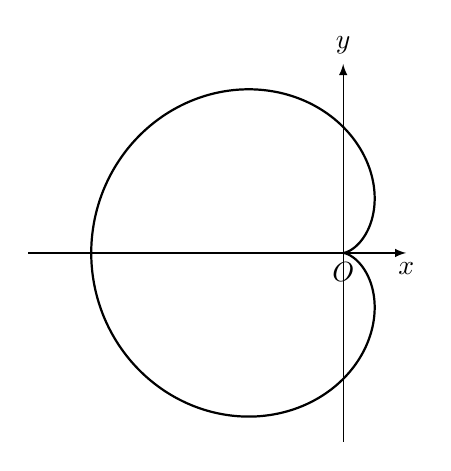
\begin{tikzpicture}[scale=0.8]
    \draw[-latex](-5,0) -- (1,0) node[below]{$x$};
    \draw[-latex](0,-3) -- (0,3) node[above]{$y$};
    \draw[black, thick, domain=0:360,smooth,variable=\t, samples=300] plot ({\t}:{2*(1-cos(\t))});
    \filldraw[black] (0,0) node[below]{$O$};
\end{tikzpicture}

水平心形线对应参数: \leavevmode \bigskip

\begin{tabular}{|c|c|c|c|c|c|c|c|c|c|}
    \hline
    $\theta$ & $0$ & $\dfrac{\pi}{6}$         & $\dfrac{\pi}{4}$         & $\dfrac{\pi}{3}$ & $\dfrac{\pi}{2}$ & $\dfrac{2\pi}{3}$ & $\dfrac{3\pi}{4}$        & $\dfrac{5\pi}{6}$        & $\pi$ \\ \hline
    $r$      & $0$ & $\dfrac{2-\sqrt{3}}{2}a$ & $\dfrac{2-\sqrt{2}}{2}a$ & $\dfrac{1}{2}a$  & $a$             & $\dfrac{3}{2}a$   & $\dfrac{2+\sqrt{2}}{2}a$ & $\dfrac{2+\sqrt{3}}{2}a$ & $2a$  \\
    \hline
\end{tabular}

\paragraph{玫瑰线} \leavevmode \bigskip

表达式:$r=a\sin(n\theta)$,周期为$\dfrac{2\pi}{n}$。

当$n$为3时为三叶,2时为四叶,$\dfrac{3}{2}$为六叶。三叶时周期为$\dfrac{2\pi}{3}$。

直角坐标系下表达式:$x=a\cdot\sin(n\cdot\theta)\cdot\cos(\theta)$与$y=a\cdot\sin(n\cdot)\cdot\sin(\theta)$

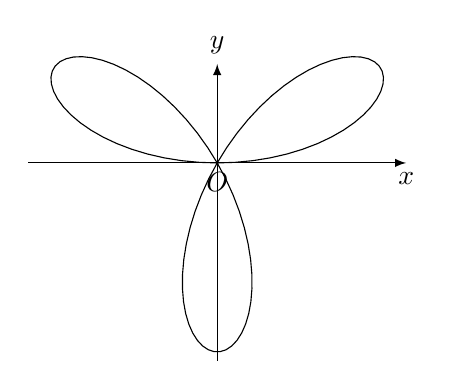
\begin{tikzpicture}[scale=0.8]
    \draw[-latex](-3,0) -- (3,0) node[below]{$x$};
    \draw[-latex](0,-pi) -- (0,pi/2) node[above]{$y$};
    \draw[domain=0:180,samples=100] plot (\x:{3*sin(\x*3)});
    \filldraw[black] (0,0) node[below]{$O$};
\end{tikzpicture}

三叶玫瑰线对应参数: \leavevmode \bigskip

\begin{tabular}{|c|c|c|c|c|c|c|c|c|c|}
    \hline
    $\theta$ & $0$ & $\dfrac{\pi}{12}$      & $\dfrac{\pi}{6}$ & $\dfrac{\pi}{4}$       & $\dfrac{\pi}{3}$ & $\dfrac{5\pi}{12}$     & $\dfrac{\pi}{2}$ & $\dfrac{7\pi}{12}$     & $\dfrac{3\pi}{2}$ \\ \hline
    $r$      & $0$ & $\dfrac{\sqrt{2}}{2}a$ & $a$             & $\dfrac{\sqrt{2}}{2}a$ & $0$             & $-frac{\sqrt{2}}{2}a$ & $-a$            & $-frac{\sqrt{2}}{2}a$ & $0$              \\
    \hline
\end{tabular}

\paragraph{阿基米德螺线} \leavevmode \bigskip

表达式:$r=a\theta$,其中$a>0$,$\theta\geqslant 0$由0开始增大时$r$也在不断增大。

\begin{tikzpicture}[scale=0.2]
    \draw[-latex](-10,0) -- (15,0) node[below]{$x$};
    \draw[-latex](0,-15) -- (0,10) node[above]{$y$};
    \draw[domain=0:720,samples=100] plot (\x:{rad(\x)});
    \filldraw[black] (0,0) node[below]{$O$};
\end{tikzpicture}

\paragraph{伯努利双扭线} \leavevmode \bigskip

设定线段$F_1F_2$长度为$2a$,伯努利双扭线上所有点M满足$MF_1\cdot MF_2=a^2$。

表达式:$r^2=2a^2\cos 2\theta$或$r^2=2a^2\sin 2\theta$。

直角坐标系下表达式:$(x^2+y^2)^2=2a^2(x^2-y^2)$。

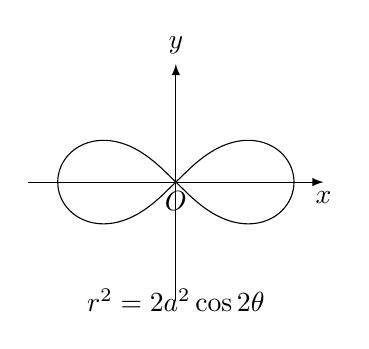
\begin{tikzpicture}[scale=1.5]
    \draw[-latex](-1.25,0) -- (1.25,0) node[below]{$x$};
    \draw[-latex](0,-1) -- (0,1) node[above]{$y$};
    \draw[domain=-45:45,samples=100] plot (\x:{sqrt(cos(\x*2))});
    \draw[domain=-45:45,samples=100] plot (\x:{-sqrt(cos(\x*2))});
    \filldraw[black] (0,0) node[below]{$O$};
    \filldraw[black] (0,-1) node{$r^2=2a^2\cos 2\theta$};
\end{tikzpicture}
\hspace{2.5em}
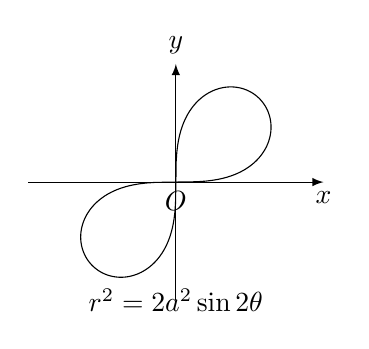
\begin{tikzpicture}[scale=1.5]
    \draw[-latex](-1.25,0) -- (1.25,0) node[below]{$x$};
    \draw[-latex](0,-1) -- (0,1) node[above]{$y$};
    \draw[domain=0:90,samples=100] plot (\x:{sqrt(sin(\x*2))});
    \draw[domain=0:90,samples=100] plot (\x:{-sqrt(sin(\x*2))});
    \filldraw[black] (0,0) node[below]{$O$};
    \filldraw[black] (0,-1) node{$r^2=2a^2\sin 2\theta$};
\end{tikzpicture}

\subsubsection{直角坐标系下画极坐标图像}

令$\theta$为$x$,令$r$为$y$。如心形线$r=2(1-\cos\theta)$:

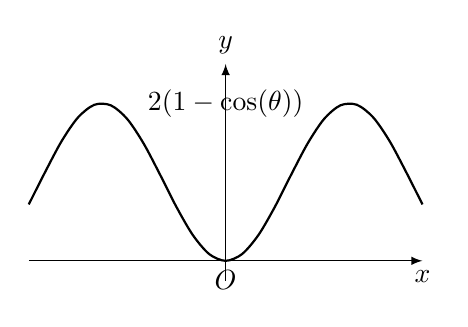
\begin{tikzpicture}[scale=0.5]
    \draw[-latex](-5,0) -- (5,0) node[below]{$x$};
    \draw[-latex](0,-0.5) -- (0,5) node[above]{$y$};
    \draw[black, thick, smooth, domain=-5:5] plot (\x,{2*(1-cos(\x r))}) node at (0,4){$2(1-\cos(\theta))$};
    \filldraw[black] (0,0) node[below]{$O$};
\end{tikzpicture}

按直角坐标系的图就可以计算出对应的$r$从而能画出对应的图像。

\subsection{参数法}

如果很难使用直角坐标或极坐标来表示曲线,那么可以引入一个新的变量参数来表示,即得到参数方程:$
    \left\{
    \begin{array}{lcl}
        x=x(t) \\
        y=y(t)
    \end{array}
    \right.
$

\subsubsection{摆线(平摆线)}

摆线,又称旋轮线、圆滚线,是一个圆沿一条直线滚动时,圆边界上一定点所形成的轨迹。

令圆半径为$r$,摆点与圆心所成直线所转动夹角对应弧度为$t$,其中$t\in[0,2\pi]$,所对应参数方程为:

$$
    \left\{
    \begin{array}{lcl}
        x=r(t-\sin t) \\
        y=r(1-\cos t)
    \end{array}
    \right.
$$

\subsubsection{星形线(内摆线)}

与半径为$r$的定圆内切的半径为$\dfrac{r}{4}$的动圆沿定圆无滑动地滚动,动圆上一点的轨迹称为星形线。

令$t$表示摆点与圆心的连线所构成夹角的弧度,其中$t\in[0,2\pi]$,得对应参数方程:

$$
    \left\{
    \begin{array}{lcl}
        x=r\cos^3t \\
        y=r\sin^3t
    \end{array}
    \right.
$$

由$\cos^2t+\sin^2t=1$得到直角坐标方程:$x^{\frac{2}{3}}+y^{\frac{2}{3}}=r^{\frac{2}{3}}$

\section{常用基础知识}
\subsection{数列}
\subsubsection{等差数列}

首项为$a_1$,公差为$d(d\neq 0)$的数列:$a_1,a_1+d,a_1+2d\cdots a_1+(n-1)d$。

通项公式:$a_n=a_1+(n-1)d$。

前$n$项和:$S_n=\dfrac{n}{2}[2a_1+(n-1)d]=\dfrac{n}{2}(a_1+a_n)$

\subsubsection{等比数列}

首项为$a_1$,公比为$q(q\neq 0)$的数列:$a_1,a_1q,a_1a^2\cdots a_1q^{n-1}$。

通项公式:$a_n=a_1q^{n-1}$。

前$n$项和:$S_n=
    \left\{
    \begin{array}{lcl}
        na_1,                   &  & r=1     \\
        \dfrac{a_1(1-r^n)}{1-r}, &  & r\neq 1
    \end{array}
    \right.$

若首项为1,则$1+r+r^2+\cdots+r^{n-1}=\dfrac{1-r^n}{1-r}(r\neq 1)$。

则对无穷的极限为$\dfrac{1}{1-r}$。

\subsubsection{常见数列前$n$项和}

\begin{enumerate}
    \item $\sum_{k=1}^nk=1+2+\cdots+n=\dfrac{n(n+1)}{2}$。
    \item $\sum_{k=1}^nk^2=1^2+2^2+\cdots+n^2=\dfrac{n(n+1)(2n+1)}{6}$。
    \item $\sum_{k=1}^n\dfrac{1}{k(k+1)}=\dfrac{1}{1\times 2}+\dfrac{1}{2\times 3}+\cdots+\dfrac{1}{n(n+1)}=\dfrac{n}{n+1}$。
\end{enumerate}

\subsection{三角函数}

\subsubsection{基本关系}

$\csc\alpha=\dfrac{1}{\sin\alpha},\sec\alpha=\dfrac{1}{\cos\alpha},\cot\alpha=\dfrac{1}{\tan\alpha},\tan\alpha=\dfrac{\sin\alpha}{\cos\alpha},\cot\alpha=\dfrac{\cos\alpha}{\sin\alpha}$。

$\sin^2\alpha+\cos^2\alpha=1,1+\tan^2\alpha=\sec^2\alpha,1+\cot^2\alpha=\csc^2\alpha$。

\subsubsection{诱导公式}

奇变偶不变,符号看象限。奇指前面添加的常数项是否为$\pi$的整数倍,是就需要改变函数,看象限指添加了常数后整体的符号看函数所在象限的符号。

\begin{enumerate}
    \item $\sin(\dfrac{\pi}{2}\pm\alpha)=\cos\alpha$
    \item $\cos(\dfrac{\pi}{2}\pm\alpha)=\mp\sin\alpha$
    \item $\sin(\pi\pm\alpha)=\mp\sin\alpha$
    \item $\cos(\pi\pm\alpha)=-\cos\alpha$
\end{enumerate}

\subsubsection{倍角公式}

$\sin 2\alpha=2\sin\alpha\cos\alpha,\cos 2\alpha=\cos^2\alpha-\sin^2\alpha=1-2\sin^2\alpha=2\cos^2\alpha-1$。

$\sin 3\alpha=-4\sin^3\alpha_3\sin\alpha,\cos 3\alpha=4\cos^3\alpha-3\cos\alpha$。

$\tan 2\alpha=\dfrac{2\tan\alpha}{1-\tan^2\alpha},\cot 2\alpha=\dfrac{\cot^2\alpha-1}{2\cot\alpha}$。

\subsubsection{半角公式}

$\sin^2\dfrac{\alpha}{2}=\dfrac{1}{2}(1-\cos\alpha),\cos^2\dfrac{\alpha}{2}=\dfrac{1}{2}(1+\cos\alpha)\text{(降幂公式)}$。

$\sin\dfrac{\alpha}{2}=\pm\sqrt{\dfrac{1-\cos\alpha}{2}},\cos\dfrac{\alpha}{2}=\pm\sqrt{\dfrac{1+\cos\alpha}{2}}$。

$\tan\dfrac{\alpha}{2}=\dfrac{1-\cos\alpha}{\sin\alpha}=\dfrac{\sin\alpha}{1+\cos\alpha}=\pm\sqrt{\dfrac{1-\cos\alpha}{1+\cos\alpha}}=\dfrac{1}{\cot\dfrac{\alpha}{2}}$。

\subsubsection{和差公式}

$\sin$和$\tan$的和差公式更容易考到。

$\sin(\alpha\pm\beta)=\sin\alpha\cos\beta\pm\cos\alpha\sin\beta,\cos(\alpha\pm\beta)=\cos\alpha\cos\beta\mp\sin\alpha\sin\beta$。

$\tan(\alpha\pm\beta)=\dfrac{\tan\alpha\pm\tan\beta}{1\mp\tan\alpha\tan\beta},\cot(\alpha\pm\beta)=\dfrac{\cot\alpha\cot\beta\mp 1}{\cot\beta\pm\cot\alpha}$。

\subsubsection{积化和差公式}

和差化积与积化和差不需要背。

$\sin\alpha\cos\beta=\dfrac{1}{2}[\sin(\alpha+\beta)+\sin(\alpha-\beta)],\cos\alpha\sin\beta=\dfrac{1}{2}[\sin(\alpha+\beta)-\sin(\alpha-\beta)]$。

$\cos\alpha\cos\beta=\dfrac{1}{2}[\cos(\alpha+\beta)+\cos(\alpha-\beta)],\sin\alpha\sin\beta=\dfrac{1}{2}[\cos(\alpha-\beta)-\cos(\alpha+\beta)]$。

\subsubsection{和差化积公式}

$\sin\alpha+\sin\beta=2\sin\dfrac{\alpha+\beta}{2}\cos\dfrac{\alpha-\beta}{2},\sin\alpha-\sin\beta=2\sin\dfrac{\alpha-\beta}{2}\cos\dfrac{\alpha+\beta}{2}$。

$\cos\alpha+\cos\beta=2\cos\dfrac{\alpha+\beta}{2}\cos\dfrac{\alpha-\beta}{2},\cos\alpha-\cos\beta=-2\sin\dfrac{\alpha+\beta}{2}\sin\dfrac{\alpha-\beta}{2}$。

\subsubsection{万能公式}

一般不会用到。

若$u=\tan\dfrac{x}{2}(-\pi<x<\pi)$,则$\sin x=\dfrac{2u}{1+u^2},\cos x=\dfrac{1-u^2}{1+u^2}$。

\subsection{指数运算法则}

$a^\alpha\cdot a^\beta=a^{\alpha+\beta},\dfrac{a^\alpha}{a^\beta}=a^{\alpha-\beta},(a^\alpha)^\beta=a^{\alpha\beta},(ab)^\alpha=a^\alpha b^\alpha,(\dfrac{a}{b})^\alpha=\dfrac{a^\alpha}{b^\alpha}$。

其中$a$,$b$为正实数,$\alpha$,$\beta$为任意实数。

\subsection{对数运算法则}

重点:

\begin{enumerate}
    \item $\log_a(MN)=\log_aM+\log_aN$(积的对数=对数的和)。
    \item $\log_a(\dfrac{M}{N})=\log_aM-\log_aN$(商的对数=对数的差)。
    \item $\log_aM^n=n\log_aM$(幂的对数=对数的倍数)。
    \item $\log_a\sqrt[n]{M}=\dfrac{1}{n}\log_aM$。
\end{enumerate}

所以以后多项相乘相除乘方开放都\textcolor{orange}{取对数}进行化简。

对于分数相减的对数先\textcolor{orange}{通分}再进行对数减法。

如下面这个题(先不要求能直接证明):

\textbf{例题4:}证明$\dfrac{1}{x+1}<\ln(1+\dfrac{1}{x})<\dfrac{1}{x}$,其中$x>0$。

首先因为证明中间项无法进行直接处理,又看到是一个对数,所以进行通分:$\ln(1+\dfrac{1}{x})=\ln\dfrac{x+1}{x}=\ln(x+1)-\ln x$。

又因为是证明该中间式在一个区间,所以很明显会想到拉格朗日中值定理:$f(b)-f(a)=f'(\xi)(b-a)$。

得到原式$=f'(\xi)=(\ln\xi)'=\dfrac{1}{\xi}$,又中值定理下$a<\xi<b$且$x>0$,所以$\dfrac{1}{b}<\dfrac{1}{\xi}<\dfrac{1}{a}$,得到$0<\dfrac{1}{x+1}<\dfrac{1}{\xi}<\dfrac{1}{x}$。

所以原式$\dfrac{1}{x+1}<\ln(1+\dfrac{1}{x})<\dfrac{1}{x}$成立。

\subsection{一元二次方程基础}

\begin{enumerate}
    \item 基本格式为$ax^2+bx+c=0(a\neq 0)$。
    \item 如果$\Delta=\sqrt{b^2-4ac}\geqslant 0$,根的公式为$x_{1,2}=\dfrac{-b\pm\sqrt{b^2-4ac}}{2a}$,其中如果等于0为唯一实根,如果大于0为二重实根,如果$\Delta<0$则得到共轭复数根$-\dfrac{b}{2a}\pm\dfrac{\sqrt{4ac-b^2}}{2a}i$。
    \item 根与系数的关系(韦达定理)为$x_1+x_2=-\dfrac{b}{a},x_1x_2=\dfrac{c}{a}$。
    \item 抛物线顶点为$(-\dfrac{b}{2a},c-\dfrac{b^2}{4a})$。
\end{enumerate}

\subsection{因式分解公式}

重点为3、4、7和11的公式。

\begin{enumerate}
    \item $(a+b)^2=a^2+2ab+b^2$。
    \item $(a-b)^2=a^2-2ab+b^2$。
    \item $(a+b)^3=a^3+3a^2b+3ab^2+b^3$。
    \item $(a-b)^3=a^3-3a^2b+3ab^2-b^3$。
    \item $a^2-b^2=(a+b)(a-b)$。
    \item $a^3-b^3=(a-b)(a^2+ab+b^2)$。
    \item $a^3+b^3=(a+b)(a^2-ab+b^2)$。
    \item $n$为正整数时,$a^n-b^n=(a-b)(a^{n-1}+a^{n-2}b+\cdots+ab^{n-2}+b^{n-1})$。
    \item $n$为正偶数时,$a^n-b^n=(a+b)(a^{n-1}-a^{n-2}b+\cdots+ab^{n-2}-b^{n-1})$。
    \item $n$为正奇数时,$a^n+b^n=(a+b)(a^{n-1}-a^{n-2}b+\cdots-ab^{n-2}+b^{n-1})$。
    \item 二项式定理$(a+b)^n=\sum_{k=0}^nC_n^ka^{n-k}b^k=a^n+na^{n-1}b+\dfrac{n(n-1)}{2!}a^{n-2}b^2+\cdots+\dfrac{n(n-1)\cdots(n-k+1)}{k!}a^{n-k}b^k+\cdots+nab^{n-1}+b^n$。
\end{enumerate}

对于二项式定理需要记忆,后面的幂比较简单,而前面的系数比较困难,可以使用杨辉三角形来记忆:


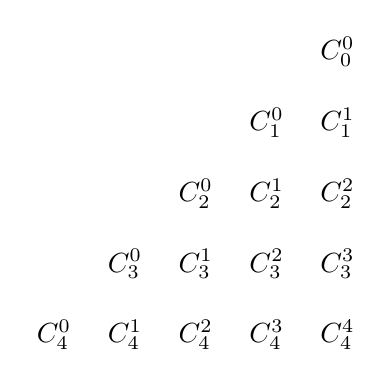
\begin{tikzpicture}[scale=0.9]
    \node[black] at (0,0) {$C_0^0$};
    \node[black] at (-1,-1) {$C_1^0$};
    \node[black] at (0,-1) {$C_1^1$};
    \node[black] at (-2,-2) {$C_2^0$};
    \node[black] at (-1,-2) {$C_2^1$};
    \node[black] at (-0,-2) {$C_2^2$};
    \node[black] at (-3,-3) {$C_3^0$};
    \node[black] at (-2,-3) {$C_3^1$};
    \node[black] at (-1,-3) {$C_3^2$};
    \node[black] at (-0,-3) {$C_3^3$};
    \node[black] at (-4,-4) {$C_4^0$};
    \node[black] at (-3,-4) {$C_4^1$};
    \node[black] at (-2,-4) {$C_4^2$};
    \node[black] at (-1,-4) {$C_4^3$};
    \node[black] at (-0,-4) {$C_4^4$};
\end{tikzpicture}
\hspace{2.5em}
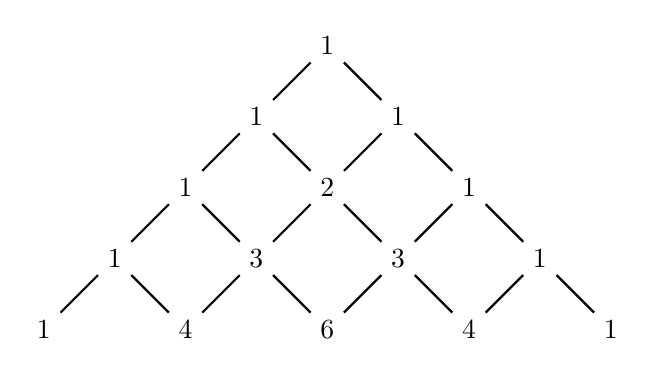
\begin{tikzpicture}[scale=0.9]
    \node[black] (0) at (0,0) {1};
    \node[black] (1) at (-1,-1) {1};
    \node[black] (2) at (1,-1) {1};
    \node[black] (3) at (-2,-2) {1};
    \node[black] (4) at (0,-2) {2};
    \node[black] (5) at (2,-2) {1};
    \node[black] (6) at (-3,-3) {1};
    \node[black] (7) at (-1,-3) {3};
    \node[black] (8) at (1,-3) {3};
    \node[black] (9) at (3,-3) {1};
    \node[black] (10) at (-4,-4) {1};
    \node[black] (11) at (-2,-4) {4};
    \node[black] (12) at (0,-4) {6};
    \node[black] (13) at (2,-4) {4};
    \node[black] (14) at (4,-4) {1};
    \draw[-,thick] (0) to (1);
    \draw[-,thick] (0) to (2);
    \draw[-,thick] (1) to (3);
    \draw[-,thick] (1) to (4);
    \draw[-,thick] (2) to (4);
    \draw[-,thick] (2) to (5);
    \draw[-,thick] (3) to (6);
    \draw[-,thick] (3) to (7);
    \draw[-,thick] (4) to (7);
    \draw[-,thick] (4) to (8);
    \draw[-,thick] (5) to (8);
    \draw[-,thick] (5) to (9);
    \draw[-,thick] (6) to (10);
    \draw[-,thick] (6) to (11);
    \draw[-,thick] (7) to (11);
    \draw[-,thick] (7) to (12);
    \draw[-,thick] (8) to (12);
    \draw[-,thick] (8) to (13);
    \draw[-,thick] (9) to (13);
    \draw[-,thick] (9) to (14);
\end{tikzpicture}

\subsection{阶乘与双阶乘}

\begin{enumerate}
    \item $n!=1\times 2\times 3\times\cdots\times n$,其中$0!=1$。
    \item $(2n)!!=2\times 4\times 6\times\cdots\times(2n)=2^n\cdot n!$。
    \item $(2n-1)!!=1\times 3\times 5\times\cdots\times(2n-1)$。
\end{enumerate}

以后的华里士公式(点火公式)会使用到,如下面的题目:

\textbf{例题5:}计算$\int_0^{\frac{\pi}{2}}\sin^{10}x\rm{d}x$与$\int_0^{\frac{\pi}{2}}\cos^9x\rm{d}x$。

原式1为偶数次幂,所以$=\dfrac{9}{10}\cdot\dfrac{7}{8}\cdot\dfrac{5}{6}\cdot\dfrac{3}{4}\cdot\dfrac{1}{2}\cdot\dfrac{\pi}{2}=\dfrac{\pi}{2}\cdot\dfrac{9!!}{10!!}$

原式2为奇数次幂,所以$=\dfrac{8}{9}\cdot\dfrac{6}{7}\cdot\dfrac{4}{5}\cdot\dfrac{2}{3}=\dfrac{8!!}{9!!}$

\subsection{常用不等式}

非常重要。

\subsubsection{绝对值不等式}

若$a$,$b$为实数,则:

\begin{enumerate}
    \item $\vert a\pm b\vert\leqslant\vert a\vert+\vert b\vert$。
    \item 推广公式一到离散区间:$\vert a_1\pm a_2\pm a_3\pm\cdots\pm a_n\vert\leqslant\vert a_1\vert+\vert a_2\vert+\cdots+\vert a_n\vert$。
    \item 推广公式一到连续区间且$f(x)$在$[a,b](a<b)$上可积:$\vert\int_a^bf(x)\rm{d}x\vert\leqslant\int_a^b\vert f(x)\vert\rm{d}x$。因为符号不一定相同的面积代数和一定小于同为正的面积代数和。
    \item $\vert\vert a\vert-\vert b\vert\vert\leqslant\vert a-b\vert$。后式子为两点之差,前式子可以看作$a$、$b$两点与0之间的距离的差,若异号则两者必然抵消一部分,若同号则就等于后式。
\end{enumerate}



\subsubsection{根号不等式}

公式一非常重要,即算数平均值大几何平均值。

$a,b,c>0$:

\begin{enumerate}
    \item $\sqrt{ab}\leqslant\dfrac{a+b}{2}\leqslant\sqrt{\dfrac{a^2+b^2}{2}}$。
    \item $\sqrt[3]{abc}\leqslant\dfrac{a+b+c}{3}\leqslant\dfrac{a^2+b^2+c^2}{3}$。
\end{enumerate}

\textbf{例题6:}证明函数$f(x)=\dfrac{x}{1+x^2}$在$(-\infty,+\infty)$内有界。

可以使用极限,若极限存在则函数有界,这里使用有界性定义与不等式来完成。

\ding{172}当$x=0$时,$f(0)=\dfrac{0}{1}$,有界。

\ding{173}当$x\neq 0$时,原式分式上下都有$x$,所以简化公式:$f(x)=\dfrac{\dfrac{x}{x}}{\dfrac{1+x^2}{x}}=\dfrac{1}{\dfrac{1}{x}+x}$。

$\because$需要证明有界性,以及根号不等式下需要参数大于0,所以需要证明$\vert f(x)\vert=\dfrac{1}{\dfrac{1}{\vert x\vert}+\vert x\vert}\leqslant M$

又$\because\dfrac{a+b}{2}\geqslant\sqrt{ab}$,$\therefore \dfrac{\dfrac{1}{\vert x\vert}+\vert x\vert}{2}\geqslant\sqrt{\dfrac{1}{\vert x\vert}\cdot\vert x\vert}=1$

$\therefore\vert f(x)\vert=\dfrac{1}{\dfrac{1}{\vert x\vert}+\vert x\vert}\leqslant\dfrac{1}{2}$。

故整个函数在$R$上有界。

\subsubsection{指数不等式}

设$a>b>0$,则$
\left\{
\begin{array}{lcl}
    a^n>b^n,   &  & \text{当}n>0\text{时} \\
    a^n<b^n, &  & \text{当}n<0\text{时}
\end{array}
\right.$。

$e^x\geqslant x+1(\forall x)$。

\subsubsection{分数不等式}

若$0<a<x<b,0<c<y<d$,则$\dfrac{c}{b}<\dfrac{y}{x}<\dfrac{d}{a}$。

\subsubsection{三角不等式}

\begin{enumerate}
    \item $\sin x<x<\tan x(0<x<\dfrac{\pi}{2})$。
    \item $\sin x<x(x>0)$。
    \item $\arctan x\leqslant x\leqslant\arcsin x(0\leqslant x\leqslant 1)$。
\end{enumerate}

\subsubsection{对数不等式}

\begin{enumerate}
    \item $x-1\geqslant\ln x(x>0)$。
    \item $\dfrac{1}{1+x}<\ln(1+\dfrac{1}{x})<\dfrac{1}{x}(x>0)$。
\end{enumerate}

\end{document}
